\documentclass[11pt,a4paper]{article}

\usepackage[T1]{fontenc}
\usepackage[utf8]{inputenc}
\usepackage{lmodern}
\usepackage[margin=2.4cm]{geometry}
\usepackage{amsmath,amssymb,amsthm,mathtools}
\usepackage{booktabs,array,tabularx}
\usepackage{enumitem}
\usepackage{xcolor}
\usepackage{tikz}
\usetikzlibrary{arrows.meta,decorations.pathreplacing,calc}
\usepackage[colorlinks=true,linkcolor=teal!70!black,citecolor=teal!70!black,urlcolor=teal!70!black]{hyperref}

\newtheorem{proposition}{Proposition}
\theoremstyle{definition}
\newtheorem{definition}{Definition}
\theoremstyle{remark}
\newtheorem{remark}{Remark}

\newcommand{\pred}{\operatorname{pred}}
\newcommand{\R}{\mathbb{R}}
\newcommand{\Pb}{\mathcal{P}}
\setlength{\parskip}{0.4em}
\setlength{\parindent}{0pt}

\title{\textbf{Scheduling a Shared XY Laser over Parallel Conveyors}\\[0.3em]
\large Formal mathematical formulation}
\author{laser-conveyor-optimization\\\small\url{https://github.com/juanlopez-gif/laser-conveyor-optimization}}
\date{November 2026 --- version 0.7.3}

\begin{document}
\maketitle

\begin{abstract}
A single Cartesian XY laser must process parts that arrive continuously on $N$
parallel conveyors. While a part is processed its conveyor stops; an unprocessed part
that reaches the end of the laser zone also stops (blocks) its conveyor. We state the
problem as an exact continuous-time model built on a \emph{belt odometer}, derive a
time-indexed mixed-integer linear program, describe the sequence-only (decoder) view
used by heuristics, discuss the online version and give structural properties and
complexity results. Every schedule produced by the simulator is checked automatically
against this model. Version 0.4.0 adds an explicit penalty for blocking events, a
pre-positioning option for the laser and a belt-order dispatching policy. Version 0.7.3
adds the information model of the controller and the general stochastic problem over a
family of cells that the learned policies target.
\end{abstract}

\tableofcontents
\bigskip

%====================================================================
\section{System and notation}
%====================================================================

\begin{figure}[h]
\centering
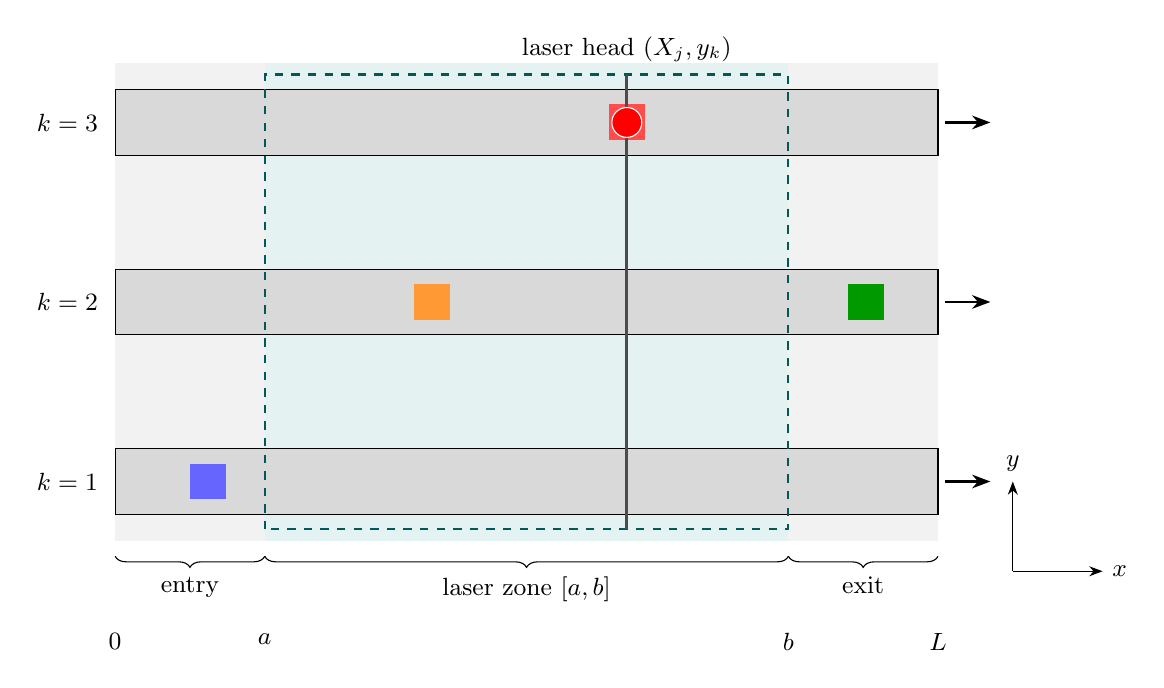
\begin{tikzpicture}[x=0.19cm,y=0.19cm,>=Stealth]
  % zones
  \fill[gray!10] (0,-4) rectangle (10,28);
  \fill[teal!10] (10,-4) rectangle (45,28);
  \fill[gray!10] (45,-4) rectangle (55,28);
  % belts
  \foreach \y/\n in {0/1,12/2,24/3}{
    \draw[fill=gray!30] (0,\y-2.2) rectangle (55,\y+2.2);
    \node[left] at (-0.5,\y) {\small $k=\n$};
    \draw[->,thick] (55.5,\y) -- (58.5,\y);
  }
  % workspace
  \draw[teal!70!black,dashed,thick] (10,-3.2) rectangle (45,27.2);
  % parts
  \fill[blue!60] (5,-1.2) rectangle (7.4,1.2);
  \fill[orange!80] (20,10.8) rectangle (22.4,13.2);
  \fill[red!70] (33,22.8) rectangle (35.4,25.2);
  \fill[green!60!black] (49,10.8) rectangle (51.4,13.2);
  % laser gantry
  \draw[very thick,gray!60!black] (34.2,-3.2) -- (34.2,27.2);
  \draw[fill=red,draw=white] (34.2,24) circle (1.0);
  \node[above] at (34.2,27.4) {\small laser head $(X_j,y_k)$};
  % axis labels
  \draw[decorate,decoration={brace,mirror,amplitude=4pt}] (0,-5) -- (10,-5)
       node[midway,below=4pt] {\small entry};
  \draw[decorate,decoration={brace,mirror,amplitude=4pt}] (10,-5) -- (45,-5)
       node[midway,below=4pt] {\small laser zone $[a,b]$};
  \draw[decorate,decoration={brace,mirror,amplitude=4pt}] (45,-5) -- (55,-5)
       node[midway,below=4pt] {\small exit};
  \node[below] at (0,-9.5) {\small $0$};
  \node[below] at (10,-9.5) {\small $a$};
  \node[below] at (45,-9.5) {\small $b$};
  \node[below] at (55,-9.5) {\small $L$};
  \draw[->] (60,-6) -- (66,-6) node[right] {\small $x$};
  \draw[->] (60,-6) -- (60,0) node[above] {\small $y$};
\end{tikzpicture}
\caption{Cell layout (top view). Parts travel in $+x$; the laser reaches the rectangle
$[a,b]\times[\min_k y_k,\max_k y_k]$.}
\end{figure}

\subsection{Sets}
\begin{tabularx}{\linewidth}{@{}l X@{}}
\toprule
$K=\{1,\dots,N\}$ & conveyors\\
$J$, $n=|J|$ & parts (jobs) of the instance\\
$J_k\subseteq J$ & parts of conveyor $k$, indexed in arrival order\\
$k(j)$ & conveyor carrying part $j$\\
$\pred(j)$ & part of $J_{k(j)}$ that arrived immediately before $j$ (none for the first)\\
\bottomrule
\end{tabularx}

\subsection{Parameters}
\begin{tabularx}{\linewidth}{@{}l X r@{}}
\toprule
symbol & meaning & default\\
\midrule
$r_j$ & arrival (release) time of part $j$ & arrival process\\
$p_j$ & processing time & $2.5$ s\\
$d_j$ & due date & $r_j+20$ s\\
$y_k$ & transverse position of conveyor $k$ & $0,12,24$ cm\\
$v_k$ & conveyor speed & $3$ cm/s\\
$a,\ b$ & start and end of the laser zone along the belt & $10,\ 45$ cm\\
$L$ & belt length (exit point) & $55$ cm\\
$\delta$ & minimum spacing between consecutive parts on a belt & $4$ cm\\
$v_x,\ v_y$ & laser axis speeds & $10,\ 10$ cm/s\\
$P_0=(x_0,y_0)$ & initial laser position & workspace centre\\
$\sigma_{kk'}\in\{0,1\}$ & $1$ if processing a part of conveyor $k'$ stops conveyor $k$ & $\sigma=I$\\
$\lambda_k$ & arrival rate of conveyor $k$ (online model) & $\tfrac1{10},\tfrac1{12},\tfrac1{14}$ s$^{-1}$\\
$G$ & distribution of the processing time (online model) & constant $2.5$ s\\
\bottomrule
\end{tabularx}

We assume $\sigma_{kk}=1$ for all $k$: a part never moves while it is processed.
The default rule $\sigma=I$ stops only the conveyor carrying the part; $\sigma\equiv 1$
stops all conveyors.

\subsection{Travel time and path length of the laser}
For $P=(x,y)$ and $Q=(x',y')$ let $\Delta x=|x'-x|$ and $\Delta y=|y'-y|$. The travel
time is
\begin{equation}\label{eq:tau}
\tau(P,Q)=
\begin{cases}
\max\!\left(\dfrac{\Delta x}{v_x},\dfrac{\Delta y}{v_y}\right) & \text{simultaneous axes (default)},\\[2ex]
\dfrac{\Delta x}{v_x}+\dfrac{\Delta y}{v_y} & \text{sequential axes}.
\end{cases}
\end{equation}
Both are metrics (weighted $\ell_\infty$ and $\ell_1$ norms), hence $\tau$ satisfies the
triangle inequality. With simultaneous axes the head moves diagonally until one axis
arrives and then straight, so the path length is
\begin{equation}\label{eq:ell}
\ell(P,Q)=\max\bigl(\Delta y+c_x\,\Delta x,\ \Delta x+c_y\,\Delta y\bigr),\qquad
c_x=\frac{\sqrt{v_x^2+v_y^2}-v_y}{v_x},\quad c_y=\frac{\sqrt{v_x^2+v_y^2}-v_x}{v_y},
\end{equation}
and $\ell=\Delta x+\Delta y$ for sequential axes. For $v_x=v_y$,
$c_x=c_y=\sqrt2-1$. Since $c_x<1$, \eqref{eq:ell} is convex in $\Delta x$ for fixed
$\Delta y$, which allows an exact linear representation in Section~\ref{sec:milp}.

%====================================================================
\section{Exact continuous-time model \texorpdfstring{$\Pb$}{P}}
%====================================================================

\subsection{Belt odometer, entry coordinates and positions}

\begin{definition}[Belt odometer]
For each conveyor $k$ let $u_k(t)\in\{0,1\}$ be its run indicator. The odometer
\[
D_k(t)=v_k\int_0^t u_k(s)\,ds
\]
is the total distance travelled by belt $k$ up to time $t$. It is continuous and
non-decreasing.
\end{definition}

All parts on a belt move rigidly with it. A part is therefore fully described by one
constant, its \emph{entry coordinate} $E_j$: the odometer reading when it is placed at
$x=0$. Because a part can only enter once the previous one has moved at least $\delta$
away from the entry,
\begin{equation}\label{eq:entry}
E_j=\max\Bigl(D_{k(j)}(r_j),\ E_{\pred(j)}+\delta\Bigr),\qquad E_{\pred(j)}:=-\infty\ \text{for the first part,}
\end{equation}
\begin{equation}\label{eq:pos}
x_j(t)=\max\bigl(0,\ D_{k(j)}(t)-E_j\bigr),\qquad t\ge r_j .
\end{equation}
The maximum in \eqref{eq:entry} models the upstream queue (state WAITING): the part
waits until the odometer reaches $E_{\pred(j)}+\delta$. The entry time is
$e_j=\min\{t\ge r_j:\ D_{k(j)}(t)\ge E_j\}$.

\subsection{Decision variables}
\begin{itemize}[nosep]
\item $\pi$: a permutation of $J$, the processing order of the laser;
\item $S_j\ge 0$: processing start time of part $j$, with $C_j=S_j+p_j$;
\item $u_k(\cdot)$: run/stop control of each conveyor (determined by the other
decisions in the non-idling model, free in the relaxed model).
\end{itemize}
Derived quantities: the \emph{processing position} and \emph{processing point}
\begin{equation}\label{eq:X}
X_j=D_{k(j)}(S_j)-E_j,\qquad P_j=(X_j,\ y_{k(j)}).
\end{equation}

\subsection{Constraints}

\paragraph{(C1) Reachability window.}
\begin{equation}\label{eq:C1}
a\le X_j\le b\qquad\forall j\in J.
\end{equation}

\paragraph{(C2) One part at a time, with travel (interception).}
\begin{equation}\label{eq:C2}
S_{\pi(1)}\ge\tau\bigl(P_0,P_{\pi(1)}\bigr),\qquad
S_{\pi(i+1)}\ge C_{\pi(i)}+\tau\bigl(P_{\pi(i)},P_{\pi(i+1)}\bigr),\quad i=1,\dots,n-1.
\end{equation}
Since $P_{\pi(i+1)}$ depends on $S_{\pi(i+1)}$ through $D_k$, inequality
\eqref{eq:C2} is \emph{implicit}: the laser, leaving $P_{\pi(i)}$ at $C_{\pi(i)}$,
reaches the point where the \emph{moving} part will be at time $S_{\pi(i+1)}$ no later
than the part (it may wait there). This is exactly the interception logic of the
simulator. By the triangle inequality, \eqref{eq:C2} implies
$S_j\ge C_i+\tau(P_i,P_j)$ for every pair with $i$ before $j$, so processing intervals
are disjoint.

\paragraph{(C3) Conveyors stop during processing.}
\begin{equation}\label{eq:C3}
u_k(t)=0\qquad\forall t\in[S_j,C_j),\ \forall j\in J\ \text{with}\ \sigma_{k\,k(j)}=1 .
\end{equation}

\paragraph{(C4) Blocking (no overrun).} An unprocessed part can never be carried
beyond $b$: $D_{k(j)}(t)-E_j\le b$ for all $t\le S_j$. Because $D_k$ is
non-decreasing this is equivalent to $X_j\le b$, i.e.\ it is already the right-hand side
of \eqref{eq:C1}. A conveyor therefore \emph{must} stop when its most downstream
unprocessed part reaches $b$.

\paragraph{(C5) Non-idling conveyors.} Conveyors normally run; a conveyor stops only
when \eqref{eq:C3} or (C4) forces it:
\begin{equation}\label{eq:C5}
u_k(t)=0\ \Longrightarrow\
\bigl(\exists j:\ \sigma_{k\,k(j)}=1,\ t\in[S_j,C_j)\bigr)\ \lor\
\bigl(\exists j\in J_k:\ S_j>t,\ D_k(t)-E_j=b\bigr).
\end{equation}
Dropping \eqref{eq:C5} yields the \emph{relaxed model} $\Pb^R$, in which conveyors may
also be stopped voluntarily (e.g.\ to keep a part inside the laser zone).

\paragraph{(C6) Workspace.} $P_j\in W=[a,b]\times[\min_k y_k,\max_k y_k]$ follows from
\eqref{eq:C1}, and straight moves between points of the convex set $W$ stay in $W$.

\subsection{Objectives}
All objectives are minimized.

\begin{center}
\begin{tabular}{@{}ll@{}}
\toprule
objective & expression\\
\midrule
makespan & $C_{\max}=\max_j C_j$\\
total flow time & $\sum_j (C_j-r_j)$\\
total waiting time & $\sum_j (S_j-r_j)$\\
maximum lateness & $L_{\max}=\max_j (C_j-d_j)$\\
laser travel distance & $\ell(P_0,P_{\pi(1)})+\sum_{i=1}^{n-1}\ell(P_{\pi(i)},P_{\pi(i+1)})$\\
conveyor downtime & $\sum_k\int_0^{T}\bigl(1-u_k(t)\bigr)dt=\sum_k\bigl(T-D_k(T)/v_k\bigr)$\\
throughput & $n/C_{\max}$ (maximizing it $\Leftrightarrow$ minimizing $C_{\max}$)\\
\bottomrule
\end{tabular}
\end{center}
Here $T$ is the time at which the last part exits ($x_j=L$).

\paragraph{Blocking penalty.} A part that reaches the end of the laser zone unprocessed
stops its \emph{whole} conveyor by (C4)--\eqref{eq:C5}: the parts behind it stop
too and no new part can enter that belt. The resulting delays are contained in $C_j$,
but a blocked conveyor has further costs in the cell (restart, accumulation upstream,
risk for the upstream process), so it is penalized explicitly. For part $j$ on conveyor
$k=k(j)$ let
\[
B_j=\min\{t:\ D_k(t)-E_j\ge b\}
\]
be the time it would reach the zone end (well defined, since by (C4) the belt
stops exactly when $x_j=b$). Part $j$ \emph{blocks} its conveyor iff it gets there
before the laser starts on it:
\begin{equation}\label{eq:block}
\beta_j=\mathbb 1[S_j>B_j],\qquad\text{blocked duration }(S_j-B_j)^+ .
\end{equation}
At most one part per conveyor (its most downstream unstarted part) can sit at $b$, and
a block lasts from $B_j$ to $S_j$, so the blocking intervals of a conveyor are disjoint.
The number of blocking events and the blocked conveyor time are
\[
N_B=\sum_j\beta_j,\qquad
T_B=\sum_j(S_j-B_j)^+=\sum_k\int_0^T\mathbb 1[\text{conveyor }k\text{ blocked at }t]\,dt ,
\]
and the blocking penalty is
\begin{equation}\label{eq:penalty}
\Pi=\lambda_N N_B+\lambda_T T_B,\qquad\lambda_N,\lambda_T\ge 0,
\end{equation}
with $\lambda_N$ in seconds per event and $\lambda_T$ in seconds per blocked
conveyor-second (defaults $10$ and $1$, placeholders until the real cost of a stopped
conveyor is known). The penalized objectives are
\[
\overline F_\Pi=\frac1n\Bigl(\sum_j F_j+\Pi\Bigr)\quad\text{(default objective)},\qquad
C_{\max}+\Pi .
\]
\emph{Attribution.} $T_B$ counts conveyor $k$ as blocked on $[B_j,S_j)$ whatever else
happens; if in that interval another part is processed and the stop rule also stops
$k$ (with $\sigma=I$: a part \emph{behind} $j$ on the same belt), the interval counts
both as blocked time and as processing downtime. $T_B$ is attributed downtime, so the
per-reason stop times may add up to more than the physical downtime.
$\overline F_\Pi$ is the total cost per part in seconds. Since $\Pi\ge 0$, every lower
bound of $\overline F$ (resp.\ $C_{\max}$) is a lower bound of $\overline F_\Pi$ (resp.\
$C_{\max}+\Pi$). The composite objective of the code is a weighted sum of these criteria,
e.g.
\[
\alpha\,C_{\max}+\beta\sum\ell+\gamma\sum_k\int_0^T(1-u_k)\,dt+\delta_W\,\overline{W}+\eta\,\overline F_\Pi ,
\]
and multi-objective studies use the Pareto front of these criteria.

\subsection{Pre-positioning and the restricted model \texorpdfstring{$\Pb^{\mathrm{sim}}$}{P-sim}}
Constraint \eqref{eq:C2} allows the laser to move towards a part \emph{before} it
reaches the laser zone (it may pre-position at $(a,y_k)$ and wait). By default the
simulator dispatches the laser only to parts that are already READY. Let
$R_j=\min\{t:\ x_j(t)\ge a\}$ be the time part $j$ enters the laser zone. The simulator
satisfies in addition
\begin{equation}\label{eq:C7}
\textbf{(C7)}\qquad S_{\pi(i+1)}\ \ge\ \max\bigl(C_{\pi(i)},\,R_{\pi(i+1)}\bigr)+\tau\bigl(P_{\pi(i)},P_{\pi(i+1)}\bigr),
\qquad S_{\pi(1)}\ge R_{\pi(1)}+\tau(P_0,P_{\pi(1)}).
\end{equation}
We write $\Pb^{\mathrm{sim}}=\Pb+\text{(C7)}$. Since (C7) only removes schedules, $\Pb$ is
a \emph{relaxation} of $\Pb^{\mathrm{sim}}$: its optimum is a lower bound for everything
the simulator can do, and the gap between both measures the value of pre-positioning
the laser. For example, a single part arriving at $t=0$ completes at $5.83$ s in $\Pb$
and at $7.19$ s in $\Pb^{\mathrm{sim}}$.

The option \texttt{laser.prepositioning} selects the model realised by the simulator:
\begin{center}
\begin{tabularx}{\linewidth}{@{}l X l@{}}
\toprule
mode & candidates when the laser is free & model\\
\midrule
\texttt{none} (default) & READY parts ($x_j\ge a$) & $\Pb^{\mathrm{sim}}$\\
\texttt{always} & READY parts and parts in the entry zone of a running belt & $\Pb$\\
\texttt{when\_idle} & entry-zone parts only if no part is READY; revoked as soon as a part becomes READY & feasible for $\Pb$\\
\bottomrule
\end{tabularx}
\end{center}
For a part in the entry zone the meeting point is searched only for $x\ge a$; the laser
goes there and waits. With \texttt{always} and a fixed sequence the simulator is the
decoder of $\Pb$: the single part above completes at $5.84$ s ($5.83$ s up to the step).
Physically, pre-positioning requires knowing that a part is in the entry zone (an entry
sensor).

\emph{Decision semantics.} Let $\mathcal R(t)$ be the READY unassigned parts and
$\mathcal U(t)$ the unassigned parts in the entry zone of a running belt. A decision
epoch is an instant at which the laser is free and the candidate set is non-empty; the
candidate set is $\mathcal R(t)$ (\texttt{none}), $\mathcal R(t)\cup\mathcal U(t)$
(\texttt{always}), or $\mathcal R(t)$ if non-empty and $\mathcal U(t)$ otherwise
(\texttt{when\_idle}). Commitments are irrevocable until processing starts, except
that under \texttt{when\_idle} a commitment to an entry-zone part $j$ is revoked at the
first instant $t'$ with $\mathcal R(t')\neq\emptyset$, $j\notin\mathcal R(t')$; the laser
keeps its position, nothing else is charged, and a new epoch occurs at $t'$ with
candidates $\mathcal R(t')$. The simulator resolves $t'$ at the granularity of its
step.

\subsection{Problem statement}
\[
(\Pb)\qquad \min_{\pi,\,S,\,u}\ f(\pi,S,u)\quad\text{s.t.}\quad
\eqref{eq:entry}\text{--}\eqref{eq:C5}.
\]

%====================================================================
\section{Time-indexed MILP \texorpdfstring{$\Pb_\Delta$}{P-Delta}}\label{sec:milp}
%====================================================================

Discretize time in steps of length $\Delta$ (e.g.\ $0.1$ s),
$t\in\mathcal T=\{0,\dots,H-1\}$, and assume $p_j=\Delta\,\bar p_j$, $r_j=\Delta\,\bar r_j$
with $\bar p_j,\bar r_j\in\mathbb Z_{\ge0}$. $M$ is a sufficiently large constant
(each big-$M$ can be tightened individually, e.g.\ to $L+v_kH\Delta$ for positions).

\subsection{Variables}
\begin{center}
\begin{tabular}{@{}lll@{}}
\toprule
variable & domain & meaning\\
\midrule
$s_{jt}$ & $\{0,1\}$ & processing of $j$ starts at step $t$\\
$u_{kt}$ & $\{0,1\}$ & conveyor $k$ runs during step $t$\\
$D_{kt}$ & $\R_{\ge0}$ & odometer of conveyor $k$ at the start of step $t$\\
$E_j,\ X_j$ & $\R$ & entry coordinate, processing position\\
$\lambda_j$ & $\{0,1\}$ & which term of the maximum defines $E_j$\\
$w_{ij}$ & $\{0,1\}$ & $i$ is processed before $j$ ($i\neq j$)\\
$\tau_{ij},\ \tau_{0j}$ & $\R_{\ge0}$ & travel times\\
$\beta_{jt}$ & $\{0,1\}$ & part $j$ blocks its conveyor at step $t$ (only for C5)\\
\bottomrule
\end{tabular}
\end{center}
$S_j:=\Delta\sum_t t\,s_{jt}$ and $C_j:=S_j+p_j$ are linear expressions.

\subsection{Constraints}
\begin{align}
&\textstyle\sum_{t\in\mathcal T}s_{jt}=1 && \forall j \tag{M1}\\
&D_{k0}=0,\qquad D_{k,t+1}=D_{kt}+v_k\Delta\,u_{kt} && \forall k,t \tag{M2}\\
&E_j\ge D_{k(j),\bar r_j},\qquad E_j\ge E_{\pred(j)}+\delta && \forall j \tag{M3a}\\
&E_j\le D_{k(j),\bar r_j}+M\lambda_j,\qquad E_j\le E_{\pred(j)}+\delta+M(1-\lambda_j) && \forall j \tag{M3b}\\
&X_j-\bigl(D_{k(j),t}-E_j\bigr)\le M(1-s_{jt}),\quad
 \bigl(D_{k(j),t}-E_j\bigr)-X_j\le M(1-s_{jt}) && \forall j,t \tag{M4}\\
&a\le X_j\le b && \forall j \tag{M5}\\
&u_{kt}+\sum_{j:\ \sigma_{k\,k(j)}=1}\ \sum_{t'=\max(0,\,t-\bar p_j+1)}^{t}s_{jt'}\le 1 && \forall k,t \tag{M6}\\
&w_{ij}+w_{ji}=1 && \forall i<j \tag{M7}\\
&S_j\ge S_i+p_i+\tau_{ij}-M(1-w_{ij}) && \forall i\neq j \tag{M8}\\
&S_j\ge\tau_{0j} && \forall j \tag{M9}
\end{align}
(M5) encodes both (C1) and the blocking constraint (C4); (M6) encodes (C3).

\paragraph{Travel times.} For simultaneous axes,
\begin{align}
&\tau_{ij}\ge\frac{X_j-X_i}{v_x},\quad \tau_{ij}\ge\frac{X_i-X_j}{v_x},\quad
\tau_{ij}\ge\frac{|y_{k(i)}-y_{k(j)}|}{v_y}, \tag{M10}\\
&\tau_{0j}\ge\frac{X_j-x_0}{v_x},\quad \tau_{0j}\ge\frac{x_0-X_j}{v_x},\quad
\tau_{0j}\ge\frac{|y_{k(j)}-y_0|}{v_y}. \tag{M11}
\end{align}
For sequential axes use $\tau_{ij}\ge\xi_{ij}/v_x+|y_{k(i)}-y_{k(j)}|/v_y$ with
$\xi_{ij}\ge\pm(X_j-X_i)$. Only lower bounds are needed: a larger $\tau$ only tightens
(M8)--(M9), so any feasible solution remains feasible when $\tau$ is lowered to the true
travel time. By the triangle inequality, imposing (M8) for all ordered pairs is
equivalent to imposing it only between consecutive parts.

\paragraph{Non-idling conveyors (C5).} Omitted for the relaxed model $\Pb^R_\Delta$:
\begin{align}
&u_{kt}\ge 1-\sum_{j:\ \sigma_{k\,k(j)}=1}\ \sum_{t'=\max(0,\,t-\bar p_j+1)}^{t}s_{jt'}-\sum_{j\in J_k}\beta_{jt} && \forall k,t \tag{M12}\\
&\beta_{jt}\le 1-\textstyle\sum_{t'\le t}s_{jt'} && \forall j,t \tag{M13}\\
&D_{k(j),t}-E_j\ge b-v_{k(j)}\Delta+\varepsilon-M(1-\beta_{jt}) && \forall j,t \tag{M14}
\end{align}
(M13) allows the blocking witness only for parts not yet started and (M14) only when the
part is \emph{strictly} inside the last step of the zone, $x_j>b-v_k\Delta$ ($\varepsilon>0$
below the position resolution): the parts that cannot advance a full step without
overshooting $b$, where the belt must stop. The slack $v_k\Delta$ is the discretization
tolerance: a conveyor may stop one step early instead of overshooting $b$ (the simulator
stops exactly at $b$ with a partial step). The threshold is strict since version 0.7.26
(an external review of Paper~1 found that with $x_j\ge b-v_k\Delta$ a part at exactly
$b-v_k\Delta$ that advances one step and starts on reaching $b$, i.e.\ $S_j=B_j$ with no
cost in the continuous model, would be charged a full event one step early); the CP-SAT
decoder already used the strict comparison.

\paragraph{Blocking witness tied to the physical state (version 0.6.0).} (M13)--(M14)
only \emph{allow} $\beta_{jt}=1$. When the belt is already stopped by a processing
operation, (M12) does not need $\beta$, so a penalized objective could set
$\beta_{jt}=0$ although $j$ sits at the zone end (external audit, 2026-11-19), whereas
the simulator and the continuous definition $(S_j-B_j)^+$ count that interval as
blocked. When $\Pi$ is in the objective we therefore add
\begin{equation}
D_{k(j),t}-E_j\le b-v_{k(j)}\Delta+M\Big(\beta_{jt}+\textstyle\sum_{t'\le t}s_{jt'}\Big)
\qquad\forall j,t \tag{M15}
\end{equation}
an unstarted part strictly inside the last step of the zone \emph{is} blocking. With
(M13)--(M15), $\beta_{jt}=1$ exactly when $j$ has not started and lies strictly within
$v_k\Delta$ of $b$, whatever the reason the belt is stopped, so $N_B$ matches the
simulator and $T_B$ up to the $O(\Delta)$ tolerance of (M14). (M15) and the penalized
objective are specified here and not implemented in the CP-SAT model (0.7.26): for the
blocking penalty this model is an approximate discretization that has not been
validated against the continuous definition.

\subsection{Objectives in linear form}
\begin{itemize}[nosep]
\item $C_{\max}\ge C_j$ and $L_{\max}\ge C_j-d_j$ for all $j$;
\item flow and waiting: $\sum_j(C_j-r_j)$ and $\sum_j(S_j-r_j)$;
\item downtime: $\Delta\sum_{k,t}(1-u_{kt})$;
\item blocking: with the variables $\beta_{jt}$ of the non-idling constraints,
$T_B=\Delta\sum_{j,t}\beta_{jt}$ and $N_B=\sum_j\gamma_j$ with $\gamma_j\in\{0,1\}$,
$\gamma_j\ge\beta_{jt}$ for all $t$, and $\Pi=\lambda_N N_B+\lambda_T T_B$, together with
(M15), which makes $\beta_{jt}$ the physical blocking indicator (without it, blocked steps
that overlap a processing stop could be dropped; corrected in version 0.6.0). (Not yet
implemented in the CP-SAT model.)
\item travel distance: add immediate-successor binaries $z_{ij}$ (with a dummy start
$0$): $\sum_i z_{ij}=1$, $\sum_j z_{ij}\le 1$, $z_{ij}\le w_{ij}$,
$w_{il}+w_{lj}\le 2-z_{ij}$ for all $l$ (nothing in between), $\xi_{ij}\ge\pm(X_j-X_i)$ and
\[
\Lambda_{ij}\ge |y_{k(i)}-y_{k(j)}|+c_x\,\xi_{ij}-M(1-z_{ij}),\qquad
\Lambda_{ij}\ge \xi_{ij}+c_y\,|y_{k(i)}-y_{k(j)}|-M(1-z_{ij}),
\]
with objective $\sum_{i,j}\Lambda_{ij}$. This is exact because $\ell$ is convex in
$\Delta x$, see \eqref{eq:ell}.
\end{itemize}

\subsection{Size}
The model has $O(nH)$ binaries $s_{jt}$, $O(NH)$ binaries $u_{kt}$ and $O(n^2)$ order
binaries. With $\Delta=0.1$ s and a $60$ s window this is a few thousand binaries for
10--15 parts, which is tractable for CP-SAT or HiGHS on small instances and inside a
rolling horizon. In CP-SAT, (M7)--(M8) are naturally written with interval variables
and \texttt{NoOverlap}, and (M4) with \texttt{AddElement} over the odometer array.

%====================================================================
\section{Sequence-only view (decoder)}
%====================================================================

Under (C5), once the order $\pi$ is fixed, the \emph{earliest} schedule compatible with
(C1)--(C5) is obtained by a deterministic forward pass: the laser leaves $P_{\pi(i)}$ at
$C_{\pi(i)}$ and heads to the earliest interception point of $\pi(i+1)$, i.e.\ the
smallest $t$ with $\tau\bigl(P_{\pi(i)},(x_{\pi(i+1)}(t),y)\bigr)\le t-C_{\pi(i)}$,
recomputed whenever a conveyor changes state; the belts evolve according to
(C3)--(C5). In the simulator the laser additionally starts towards $\pi(i+1)$ only
once that part is READY, i.e.\ the pass respects \eqref{eq:C7}. This map
$\Phi:\pi\mapsto(S,u)$, the earliest schedule of $\Pb^{\mathrm{sim}}$ for the order $\pi$,
is exactly what the simulator computes with the \texttt{fixed\_sequence} policy, hence
\[
\min_{\pi\in\mathfrak S_n} f\bigl(\Phi(\pi)\bigr)
\]
is a permutation problem that genetic algorithms, simulated annealing, tabu search or
exhaustive search (small $n$) can attack with the simulator as evaluator.

\begin{remark}
Positions depend on start times, so delaying a start can move a part closer to the
laser. The earliest (semi-active) schedule is therefore not guaranteed to dominate for
every objective: $\Phi$ is a heuristic restriction of $\Pb^{\mathrm{sim}}$ (and of
$\Pb$), while $\Pb_\Delta$ explores all start times and pre-positioning.
\end{remark}

\begin{remark}
Dynamic programming over states (processed set, last part) is \emph{not} exact: the
odometers $D_k$ depend on the whole history, so they would have to be part of the state.
\end{remark}

%====================================================================
\section{Online version}
%====================================================================

In the real cell $r_j$ (and possibly $p_j$) is revealed only when the part arrives. A
\emph{policy} maps the information available at a decision epoch (laser free) to the
next part. The offline problem $\Pb$ with full knowledge of the future gives the
\emph{clairvoyant} benchmark $f^\ast$, and a policy $\mu$ is evaluated by its expected
performance over the arrival distribution and by the empirical ratio
$\mathbb E[f(\mu)]/\mathbb E[f^\ast]$ on generated instances.

With \texttt{laser.prepositioning: none} (the default until 0.7.6; the design cell runs \texttt{when\_idle} since 0.7.7) the implemented policies satisfy
\eqref{eq:C7} (the laser only selects parts already inside the laser zone) and never
wait deliberately; they produce feasible solutions of $\Pb^{\mathrm{sim}}\subseteq\Pb$.
With pre-positioning they produce feasible solutions of $\Pb$. In every case the optimum
of $\Pb$, and every valid lower bound of $\Pb$, bounds all of them.

\emph{Belt-order policy.} Processing a conveyor out of belt order lets the earlier part
travel on towards $b$ and block. The policy \texttt{nearest\_head} only considers the
\emph{head} of every conveyor (its most downstream unstarted part) and picks the head
with the smallest interception time, so its schedules keep belt order inside every
conveyor, the structure of the good sequences found by the metaheuristics.

\emph{Reinforcement learning.} The online problem is a semi-Markov decision process:
decision epochs are the instants at which the laser is free and there are at least two
candidates (a single candidate is taken without a decision). In the 0.5--0.6 agents the
action is the conveyor whose head is served (a restricted class); in the strong-RL model
of version 0.7 the action is any candidate part. The cost accrued between epochs $t$
and $t'$ is
\[
c(t,t')=\int_t^{t'}\bigl|\{j:\ r_j\le s<C_j\}\bigr|\,ds+\lambda_T\,T_B(t,t')+\lambda_N\,N_B(t,t'),
\]
and since $\int_0^\infty|\{j:r_j\le s<C_j\}|\,ds=\sum_jF_j$, the undiscounted return of
an episode equals $-(\sum_jF_j+\Pi)=-n\,\overline F_\Pi$.

\emph{Rolling horizon:} at each decision epoch, solve $\Pb_\Delta$ restricted to the
observable parts (\S\ref{sec:info}, plus forecast arrivals, if any) over a window of $H$
steps, apply the first decision and re-solve at the next epoch.

\emph{Tie-break.} Rules that rank candidates by travel time compare the times rounded to
$10^{-9}$\,s and break exact ties by the instant from which the part has been observable
($o_j$, \S\ref{sec:info}), then by part number (version 0.7.26; up to 0.7.25 the second
key was the arrival time $r_j$, which the \texttt{belts} and \texttt{zone} levels do not
observe; the audit of the change is in \texttt{docs/methods/tiebreak\_audit.md}). Exact
ties are frequent (equal moves $\Delta y/v_y$, several parts stopped at $b$), so the tie
rule is part of the definition of a policy, and it must use observable quantities only.

\subsection{Information model}\label{sec:info}
A policy may use only what the cell observes. Let $O(t)\subseteq J$ be the parts
observable at $t$ and $o_j$ the instant from which part $j$ is observable (its arrival
$r_j$ with \texttt{full}, its entry in the visible stretch of the belt with
\texttt{belts}, its entry in the laser zone $R_j$ with \texttt{zone}). With
\texttt{belts} the camera sees the laser zone and the last $\ell_v$ cm of the entry
zone, $[a-\ell_v,a)$ (\texttt{simulation.visible\_length}, version 0.7.10); the design
camera has $\ell_v=$ \texttt{entry\_length} and sees the whole belt, so $o_j=e_j$;
$\ell_v=0$ coincides with \texttt{zone}. The information at a decision epoch is
\[
\mathcal I_t=\Bigl(t,\ \text{laser state},\ \text{belt states},\
\bigl\{(k(j),x_j(t),o_j,p_j,\text{status}_j):\ j\in O(t)\bigr\},\ \theta,\ T_A\Bigr),
\]
where $\theta$ are the cell parameters (\S\ref{sec:general}) and $T_A$ the arrival
horizon, known statistically and not an observation: the controller knows the rates
$\lambda_k$ but not the instants of the future arrivals, nor whether any part will still
arrive before $T_A$. A policy maps $\mathcal I_t$ to a candidate; a look-ahead may
simulate only the parts of $O(t)$ plus synthetic arrivals drawn from $\theta$, never the
real future. Under \texttt{belts} the arrival time $r_j$ itself is not observed: a part
that waited in the hidden upstream queue shows no trace of it (0.7.7). For the
objectives this costs nothing, since $\sum_j F_j=\sum_j C_j-\sum_j r_j$ and the $r_j$
are constants.

\begin{center}
\begin{tabularx}{\linewidth}{@{}l >{\raggedright\arraybackslash}X >{\raggedright\arraybackslash}p{0.3\linewidth}@{}}
\toprule
level & $O(t)$ & use\\
\midrule
\texttt{belts} & parts on a belt in the laser zone or in the visible stretch $[a-\ell_v,a)$ of the entry zone, with their positions & \textbf{design cell} with $\ell_v=$ \texttt{entry\_length}: an overhead camera sees every belt and its working area; shorter $\ell_v$ for the value-of-information study\\
\texttt{zone} & parts in the laser zone only & what-if without camera; incompatible with pre-positioning\\
\texttt{full} & also parts waiting upstream of the belt entry & what-if upper bound; implicit in every version before 0.7.3\\
\bottomrule
\end{tabularx}
\end{center}

Up to version 0.7.2 the look-ahead policies and the reinforcement-learning observations
also used the parts waiting upstream, which the real cell does not see. Version 0.7.3
removes them, and the tests check that changing unobservable parts never changes a
decision. The rules \texttt{nearest\_job}, \texttt{nearest\_head}, \texttt{fifo} and
\texttt{weighted\_score} choose among candidates only, which are always observable. The
processing time $p_j$ is assumed known once the part is observed (it is constant in the
real cell). Whether the laser may be \emph{sent} to an entry-zone part is a separate
question (\texttt{laser.prepositioning}); since the camera sees the entry zone, the
design cell runs \texttt{when\_idle} (version 0.7.7) and \texttt{none} is the variant
without entry detection.

\subsection{The general stochastic problem}\label{sec:general}
The learned policies target a family of cells. A cell is the parameter vector
\begin{multline*}
\theta=\bigl(N,\ (y_k,v_k,\lambda_k)_{k=1}^N,\ G,\ v_x,v_y,\ \text{motion model},\\
a,b,L,\delta,\ \sigma,\ \lambda_N,\lambda_T,\ \text{pre-positioning},\ \text{observation level}\bigr).
\end{multline*}
Given $\theta$, the arrivals of conveyor $k$ form a Poisson process of rate $\lambda_k$
(or a deterministic one of period $1/\lambda_k$, or, from version 0.7.10, an on/off
Poisson source with the same mean rate: on a fraction $f_k$ of the time in periods of
mean $\tau_k$, emitting at rate $\lambda_k/f_k$ while on, hyper-exponential
inter-arrival times), independent between conveyors. The controller knows $\lambda_k$;
$(f_k,\tau_k)$ enter $\theta$ only in the bursty regimes of the bench. The
processing times are i.i.d.\ with distribution $G$ (constant, uniform or truncated
normal). An instance $\omega$ is a realization up to the arrival horizon $T_A$, after
which the system drains. For a policy $\mu$,
\[
J(\mu;\theta)=\mathbb E_\omega\bigl[\overline F_\Pi(\mu;\theta,\omega)\bigr],\qquad
\min_\mu\ \mathbb E_{\theta\sim\Theta}\Bigl[J(\mu;\theta)\,/\,J(\mu_{\mathrm{NJ}};\theta)\Bigr],
\]
where the policy receives $\theta$ as input and the ratio to \texttt{nearest\_job} on the
same instance (common random numbers) makes cells of different scale comparable.
$J$ is estimated by the mean over seeds of the paired per-episode ratio, with a normal
95\,\% confidence interval.

\emph{Load and stability.} The processing load is $\rho_p=\sum_k\lambda_k\mathbb E[p]$.
The effective laser load $\rho=\sum_k\lambda_k(\mathbb E[p]+\bar\tau)$ also includes the
mean travel time $\bar\tau$ per part, which depends on the policy. If $\rho\ge 1$ the
queues grow without bound: finite episodes with drain stay well defined, a long-run
average does not. The real cell has $\rho_p=0.64$ and $\rho\approx0.9$ (stable); the
heavy example has $\rho_p=0.93$ and is overloaded. The training distribution draws
$\rho_p\in[0.3,0.95]$ and therefore deliberately includes overloaded cells.

\emph{Not covered by $\theta$ yet:} a processing-time distribution per conveyor or per
part type, laser acceleration, and the \texttt{pass} rule in the exact simulator.

%====================================================================
\section{Structural properties and complexity}
%====================================================================

\begin{proposition}[Rigid belts]
On each conveyor the order of the parts never changes and, once two parts $i$ (earlier)
and $j$ have entered, $x_i(t)-x_j(t)=E_j-E_i\ge\delta$. The laser may nevertheless
process them in any order.
\end{proposition}

\begin{proposition}[Blocking cascade]
On conveyor $k$ at time $t$ the binding cap is set by the most downstream unstarted part:
\[
D_k(t)\le\min\{E_j+b:\ j\in J_k,\ S_j>t\}.
\]
Processing the parts of a conveyor out of belt order therefore tends to cause
blocking.
\end{proposition}
\begin{remark}
Belt order is nevertheless \emph{not} dominant: on small instances with bursts of
arrivals the best order sometimes serves a later part of a conveyor first (gaps of a
few per cent, \texttt{docs/methods/restriction\_gap.md}). Head-only policies form a
restricted policy class.
\end{remark}

\begin{proposition}[Feasibility]
With blocking, $\Pb$ is always feasible. Even if $v_k\ge v_x$, so that the laser
cannot catch a part ahead of it while it moves, the part stops at $b$ by (C4) and is
then reachable.
\end{proposition}

\begin{proposition}[Lower bounds on the makespan]
Every feasible schedule satisfies
\[
C_{\max}\ge\max_j\Bigl(r_j+\frac{a}{v_{k(j)}}+p_j\Bigr),\qquad
C_{\max}\ge\min_j\Bigl(r_j+\frac{a}{v_{k(j)}}\Bigr)+\sum_j p_j .
\]
\end{proposition}
\begin{proof}
Part $j$ cannot reach $x=a$ before $r_j+a/v_{k(j)}$, giving the first bound. No
processing can start before the earliest such time, and processing intervals are
disjoint by (C2), giving the second.
\end{proof}
Adding a lower bound on the travel between consecutive processing points (e.g.\
$|y_k-y_{k'}|/v_y$ for every change of conveyor) strengthens the second bound.

\begin{proposition}[Complexity]
With the stop rule $\sigma=I$ and the number of conveyors $N$ part of the input, the
decision versions of $\Pb$ for $L_{\max}$ and for $\sum_jC_j$ (equivalently $\sum_jF_j$)
are NP-hard in the strong sense.
\end{proposition}
\begin{proof}
Reduce from $1\,|\,r_j\,|\,L_{\max}$ and $1\,|\,r_j\,|\,\sum C_j$ with integer data
(Lenstra, Rinnooy Kan and Brucker, 1977; the 1975 preprint BW~43/75 of the
Mathematisch Centrum proves their NP-completeness by reductions from KNAPSACK, its
Theorem~4(a) and~4(c), i.e.\ ordinary NP-hardness; the strong NP-hardness used here is
attributed to the published 1977 version, whose theorem numbers have not been checked
against that version, version 0.7.26). The reduction below preserves the encoding of
the numbers up to a polynomial factor, so the problem inherits the hardness of its
source. Given $n$ jobs $(r_j,p_j,d_j)$,
build $N=n$ conveyors of equal speed $v$, one part per conveyor, and scale by an integer
$M$: $r'_j=Mr_j$, $p'_j=Mp_j$, $d'_j=Md_j+c$ with $c=a/v$. Part $j$ reaches $x=a$ at
$Mr_j+c$. With one part per conveyor and $\sigma=I$ no belt stop delays another part, and
blocking only makes an unprocessed part wait at $b$, so the laser is the only coupling.
Every travel time is at most
$\tau_{\max}=\max\bigl((b-a)/v_x,\,(\max_ky_k-\min_ky_k)/v_y\bigr)$, polynomial in $n$.
Following an order $\pi$ and starting as early as possible gives
$C'_j\le M\,C_j(\pi)+c+n\tau_{\max}$; conversely every feasible schedule with order
$\pi$ has $C'_j\ge M\,C_j(\pi)+c$, where $C_j(\pi)$ is the non-delay schedule of $\pi$ in
the source instance. With $M>n^2\tau_{\max}$ the thresholds $ML+n\tau_{\max}$ and
$MK+nc+n^2\tau_{\max}$ separate the integer-valued source answers, and all numbers stay
polynomially bounded.
\end{proof}
\begin{remark}
Not covered: a \emph{fixed} number of conveyors (e.g.\ $N=3$), where parts share belts
and their availability depends on earlier stops, and the all-conveyors stop rule. The
makespan version is not claimed. Exact methods are realistic only for small instances
or inside a rolling horizon.
\end{remark}

In Graham-style notation the problem is
\[
1\ \big|\ r_j,\ s_{ij}(t,z),\ \text{blocking},\ \text{endogenous windows}\ \big|\ C_{\max},\ \textstyle\sum F_j,\ L_{\max},
\]
where the travel setup $s_{ij}(t,z)$ depends on the sequence, the time and the belt
state $z$ (the odometers, i.e.\ all earlier stops), because the meeting point is the
part's position at interception; the accessibility windows of a part are induced by
the belt state and hence by the schedule itself.

%====================================================================
\section{Correspondence with the simulator}
%====================================================================

\begin{center}
\begin{tabularx}{\linewidth}{@{}>{\raggedright\arraybackslash}p{0.34\linewidth} X@{}}
\toprule
model element & simulator (\texttt{src/})\\
\midrule
odometer $D_k(t)$ & \texttt{Conveyor.displacement}\\
$E_j$, $D_k(r_j)$, $D_k(S_j)$, $D_k(C_j)$, $X_j$ & \texttt{Part.entry\_coordinate}, \texttt{arrival\_displacement}, \texttt{start\_displacement}, \texttt{completion\_displacement}, \texttt{processing\_x} (exported in \texttt{parts.csv})\\
upstream queue and spacing \eqref{eq:entry} & \texttt{Conveyor.can\_admit}, \texttt{Conveyor.admit}\\
(C1) window & candidates are READY parts (plus entry-zone parts with pre-positioning); processing starts on contact inside $[a,b]$\\
(C7), pre-positioning & \texttt{laser.prepositioning}, \texttt{Simulation.\_dispatch}, \texttt{\_revoke\_prepositioning}\\
(C2) interception & \texttt{motion.find\_intercept} and re-planning in \texttt{Simulation.\_drive\_laser}\\
(C3) stop rule $\sigma$ & \texttt{stop\_policy.py}\\
(C4)--(C5) blocking, non-idling & \texttt{Conveyor.advance(block\_unprocessed=True)}, \texttt{\_update\_blocking}\\
$\tau$, $\ell$ & \texttt{motion.travel\_time}, \texttt{Laser.move\_towards}\\
$B_j$, $\beta_j$, $N_B$, $T_B$, $\Pi$ & \texttt{Part.block\_time}, \texttt{Part.caused\_block}, summary keys \texttt{blocking\_events}, \texttt{total\_blocked\_time}, \texttt{blocking\_penalty}\\
objectives & \texttt{metrics.summarize}, \texttt{optimization/objective\_functions.py}\\
information model $O(t)$ & \texttt{simulation.observation}; \texttt{Simulation.observable}, \texttt{FastSim.observable}; enforced in \texttt{policies/rollout.py}, \texttt{rl/features.py}, \texttt{rl2/}\\
exact continuous-time realisation (block mode) & \texttt{src/fastsim/} (event driven): checker tolerance $10^{-6}$; the fixed-step engine converges to it as the step goes to $0$\\
\bottomrule
\end{tabularx}
\end{center}

\texttt{optimization/schedule\_check.py} takes a simulated run and verifies
\eqref{eq:entry}, \eqref{eq:X}, \eqref{eq:C1}, \eqref{eq:C2} for every consecutive pair,
(C3) through $D_k(C_j)=D_k(S_j)$, and the belt-kinematics bound
$D_k(S_j)-D_k(S_i)\le v_k\cdot(\text{running time})$, with tolerances of the order of the
simulator step. The tests run it for every policy, for stochastic instances, for an
overloaded instance where blocking occurs and for the all-conveyors stop rule. Every
schedule produced by a policy is therefore feasible for $\Pb$ (up to the step), and an
optimal solution of $\Pb$ or $\Pb_\Delta$ is a valid benchmark for the policies.

\begin{thebibliography}{9}
\bibitem{lenstra77} J.K.~Lenstra, A.H.G.~Rinnooy Kan and P.~Brucker.
Complexity of machine scheduling problems.
\emph{Annals of Discrete Mathematics}, 1:343--362, 1977.
\bibitem{graham79} R.L.~Graham, E.L.~Lawler, J.K.~Lenstra and A.H.G.~Rinnooy Kan.
Optimization and approximation in deterministic sequencing and scheduling: a survey.
\emph{Annals of Discrete Mathematics}, 5:287--326, 1979.
\end{thebibliography}

\end{document}
